\documentclass{article}

\input tutorial_setup.tex

% use convert -density 300 *.pdf *.png

\begin{document}

\tikzsetnextfilename{04_supercell}
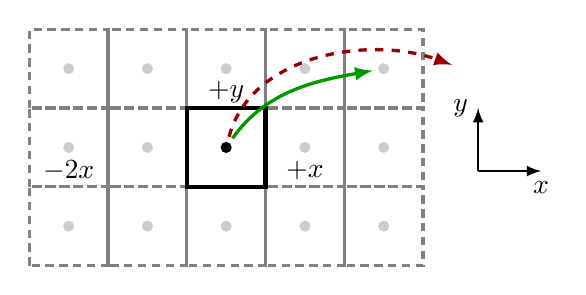
\begin{tikzpicture}[very thick, >=latex]

  \foreach \y in {-1,0,1} {
      \foreach \x in {-2,-1,0,1,2} {
          \fill[white!80!black] (0.5cm+\x cm,0.5cm +\y cm) circle (2pt);
          \draw[densely dashed,gray] (\x, \y) rectangle ++(1,1);
      }
  }
  \fill (0.5cm,0.5cm) circle (2pt);
  \draw[ultra thick] (0,0) rectangle ++(1,1);
  
  \node at (1.5,.2) {$+x$};
  \node at (-1.5,.2) {$-2x$};
  \node at (.5,1.2) {$+y$};
  
  \draw[->,shorten >=4pt, shorten <=4pt,
  green!60!black] (0.5, 0.5) to[out=55,in=190] ++(2,1);
  
  \draw[->,shorten >=4pt, shorten <=4pt,dashed,
  red!60!black] (0.5, 0.5) to[out=75,in=160] ++(3,1);
  
  \draw[thick,->] (3.7, 0.2) -- +(0.8,0) node[below] {$x$};
  \draw[thick,->] (3.7, 0.2) -- +(0,0.8) node[left] {$y$};
  
\end{tikzpicture}


\tikzsetnextfilename{04_graphene_couplings}
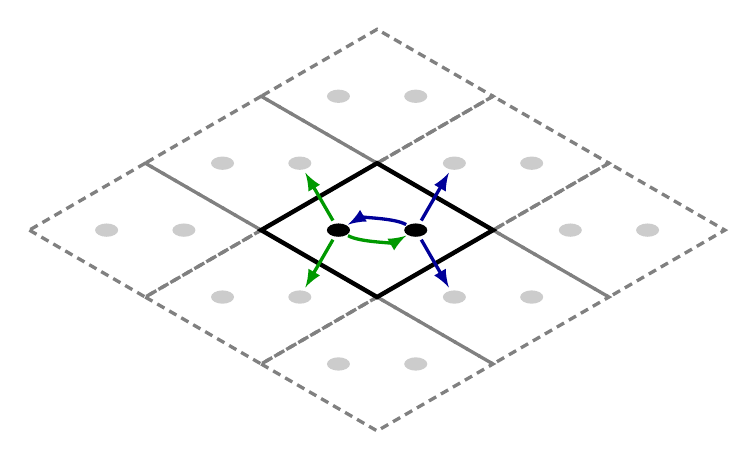
\begin{tikzpicture}[scale=1.7,very thick, >=latex, g/.style={
      cm={0.8660254, 0.5, 0.8660254, -0.5,(0,0)},
  },
  c/.style={->,shorten <=4pt, shorten >=4pt}]

  \def\xa{0.33333333}
  \def\ya{0.66666666}
  
  \foreach \y in {-1,0,1} {
      \foreach \x in {-1,0,1} {
          \fill[g,white!80!black] (\xa cm+\x cm,\xa cm +\y cm) circle (2pt);
          \fill[g,white!80!black] (\ya cm +\x cm, \ya cm +\y cm) circle (2pt);
          \draw[g,densely dashed,gray] (\x, \y) rectangle ++(1,1);
      }
  }
  \foreach \x in {\xa,\ya}{
      \fill[g] (\x,\x) circle (2pt);
  }
  \draw[g,ultra thick] (0,0) rectangle ++(1,1);

  % Draw couplings from first atom
  \draw[g,c,green!60!black] (\xa,\xa) to (\ya,\ya cm -1cm);
  \draw[g,c,green!60!black] (\xa,\xa) to[out=90,in=180,relative=false] (\ya,\ya);
  \draw[g,c,green!60!black] (\xa,\xa) to (\ya cm -1cm,\ya);

  % Draw couplings from second atom
  \draw[g,c,blue!60!black] (\ya,\ya) to (\xa,\xa cm +1cm);
  \draw[g,c,blue!60!black] (\ya,\ya) to[out=-90,in=0,relative=false] (\xa,\xa);
  \draw[g,c,blue!60!black] (\ya,\ya) to (\xa cm + 1cm,\xa);

\end{tikzpicture}

\end{document}
